%!TEX root = ../thesis.tex
%*******************************************************************************
%*********************************** First Chapter *****************************
%*******************************************************************************

\chapter{Introduction}  %Title of the First Chapter

\ifpdf
    \graphicspath{{Chapter1/Figs/Raster/}{Chapter1/Figs/PDF/}{Chapter1/Figs/}}
\else
    \graphicspath{{Chapter1/Figs/Vector/}{Chapter1/Figs/}}
\fi

\newcommand{\citetex}[1]{\citeauthor{#1} (\citeyear{#1})}
\newcommand{\citebrac}[1]{(\citeauthor{#1}, \citeyear{#1})}

%********************************** %Background  ****************************
\section{Background}

Casting bored piles and diaphragm walls in-situ {\bfseries figure \ref{fig:tremie_blank}}, requires a specialist concrete termed 'tremie concrete'. In both fresh and cured state, this concrete must meet stringent Euro and British design codes. Despite these regulations however, problems within the final product are still prevalent throughout the industry. In 2014 the European Federation of Foundation Contractors and the Deep Foundation Institute set up a task-group wherein the primary aim was to develop a clearer understanding of the root cause of these issues. The task group hypothesised that inadequate workability and stability of the concrete was in part caused by the inability of current design guidelines to predict when problems are likely to occur, \citetex{EFFC}.\\

\noindent
In order to provide evidence to support this hypothesis, two avenues of investigation have arisen. Namely, a practical approach as seen by \citet{bjorn}  and a simulative approach as described in this paper.\\

\noindent
Along side an analysis of the issues to be investigated, a comprehensive review of literature surrounding fresh concrete and its ability to be modelled accurately is presented, followed by a potential methodology of investigation. 

\begin{figure}[H]
\centering
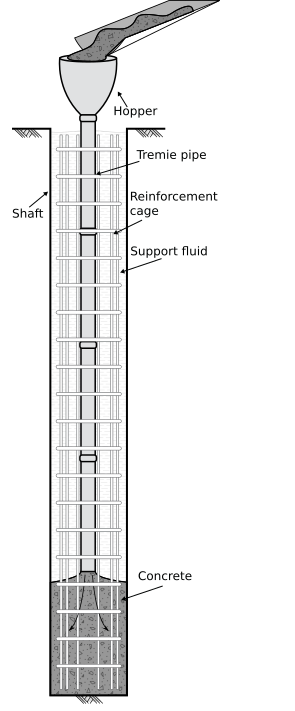
\includegraphics[width=0.4\textwidth]{tremie_empty.png}
\caption{\label{fig:tremie_blank} Schematic diagram of the tremie method for casting bored piles in situ.}
\end{figure}

\section{Research Objectives}
Coalescing all issues relating to tremie concrete into the same simulation is unlikely to produce any significant findings. A more pragmatic approach would be to assess each identified variable in the process individually, making a judgement it's impact on the final result.\\

\noindent
In this study, the impact of tremie method equipment shown in {\bfseries figure \ref{fig:tremie_blank}} is considered along side the resultant behaviour of the concrete, especially its dominant flow pattern. The change in behaviour of the concrete with changing variables will be documented in order to advise how best to avoid any issues that arise. Although there are some areas of investigation involving the tremie pipe, the dimensions and centring of the pipe as specified by EN 1536:2010 are not considered. 

%********************************** AOI  ****************************
\section{Areas of Investigation}

When analysing the tremie method, each area of investigation falls within one of three subdivisions; initiation of concrete flow, during concrete flow, and bleed and segregation, {\bfseries figure \ref{fig:tremie_colour}}.

\begin{figure}[H]
\centering
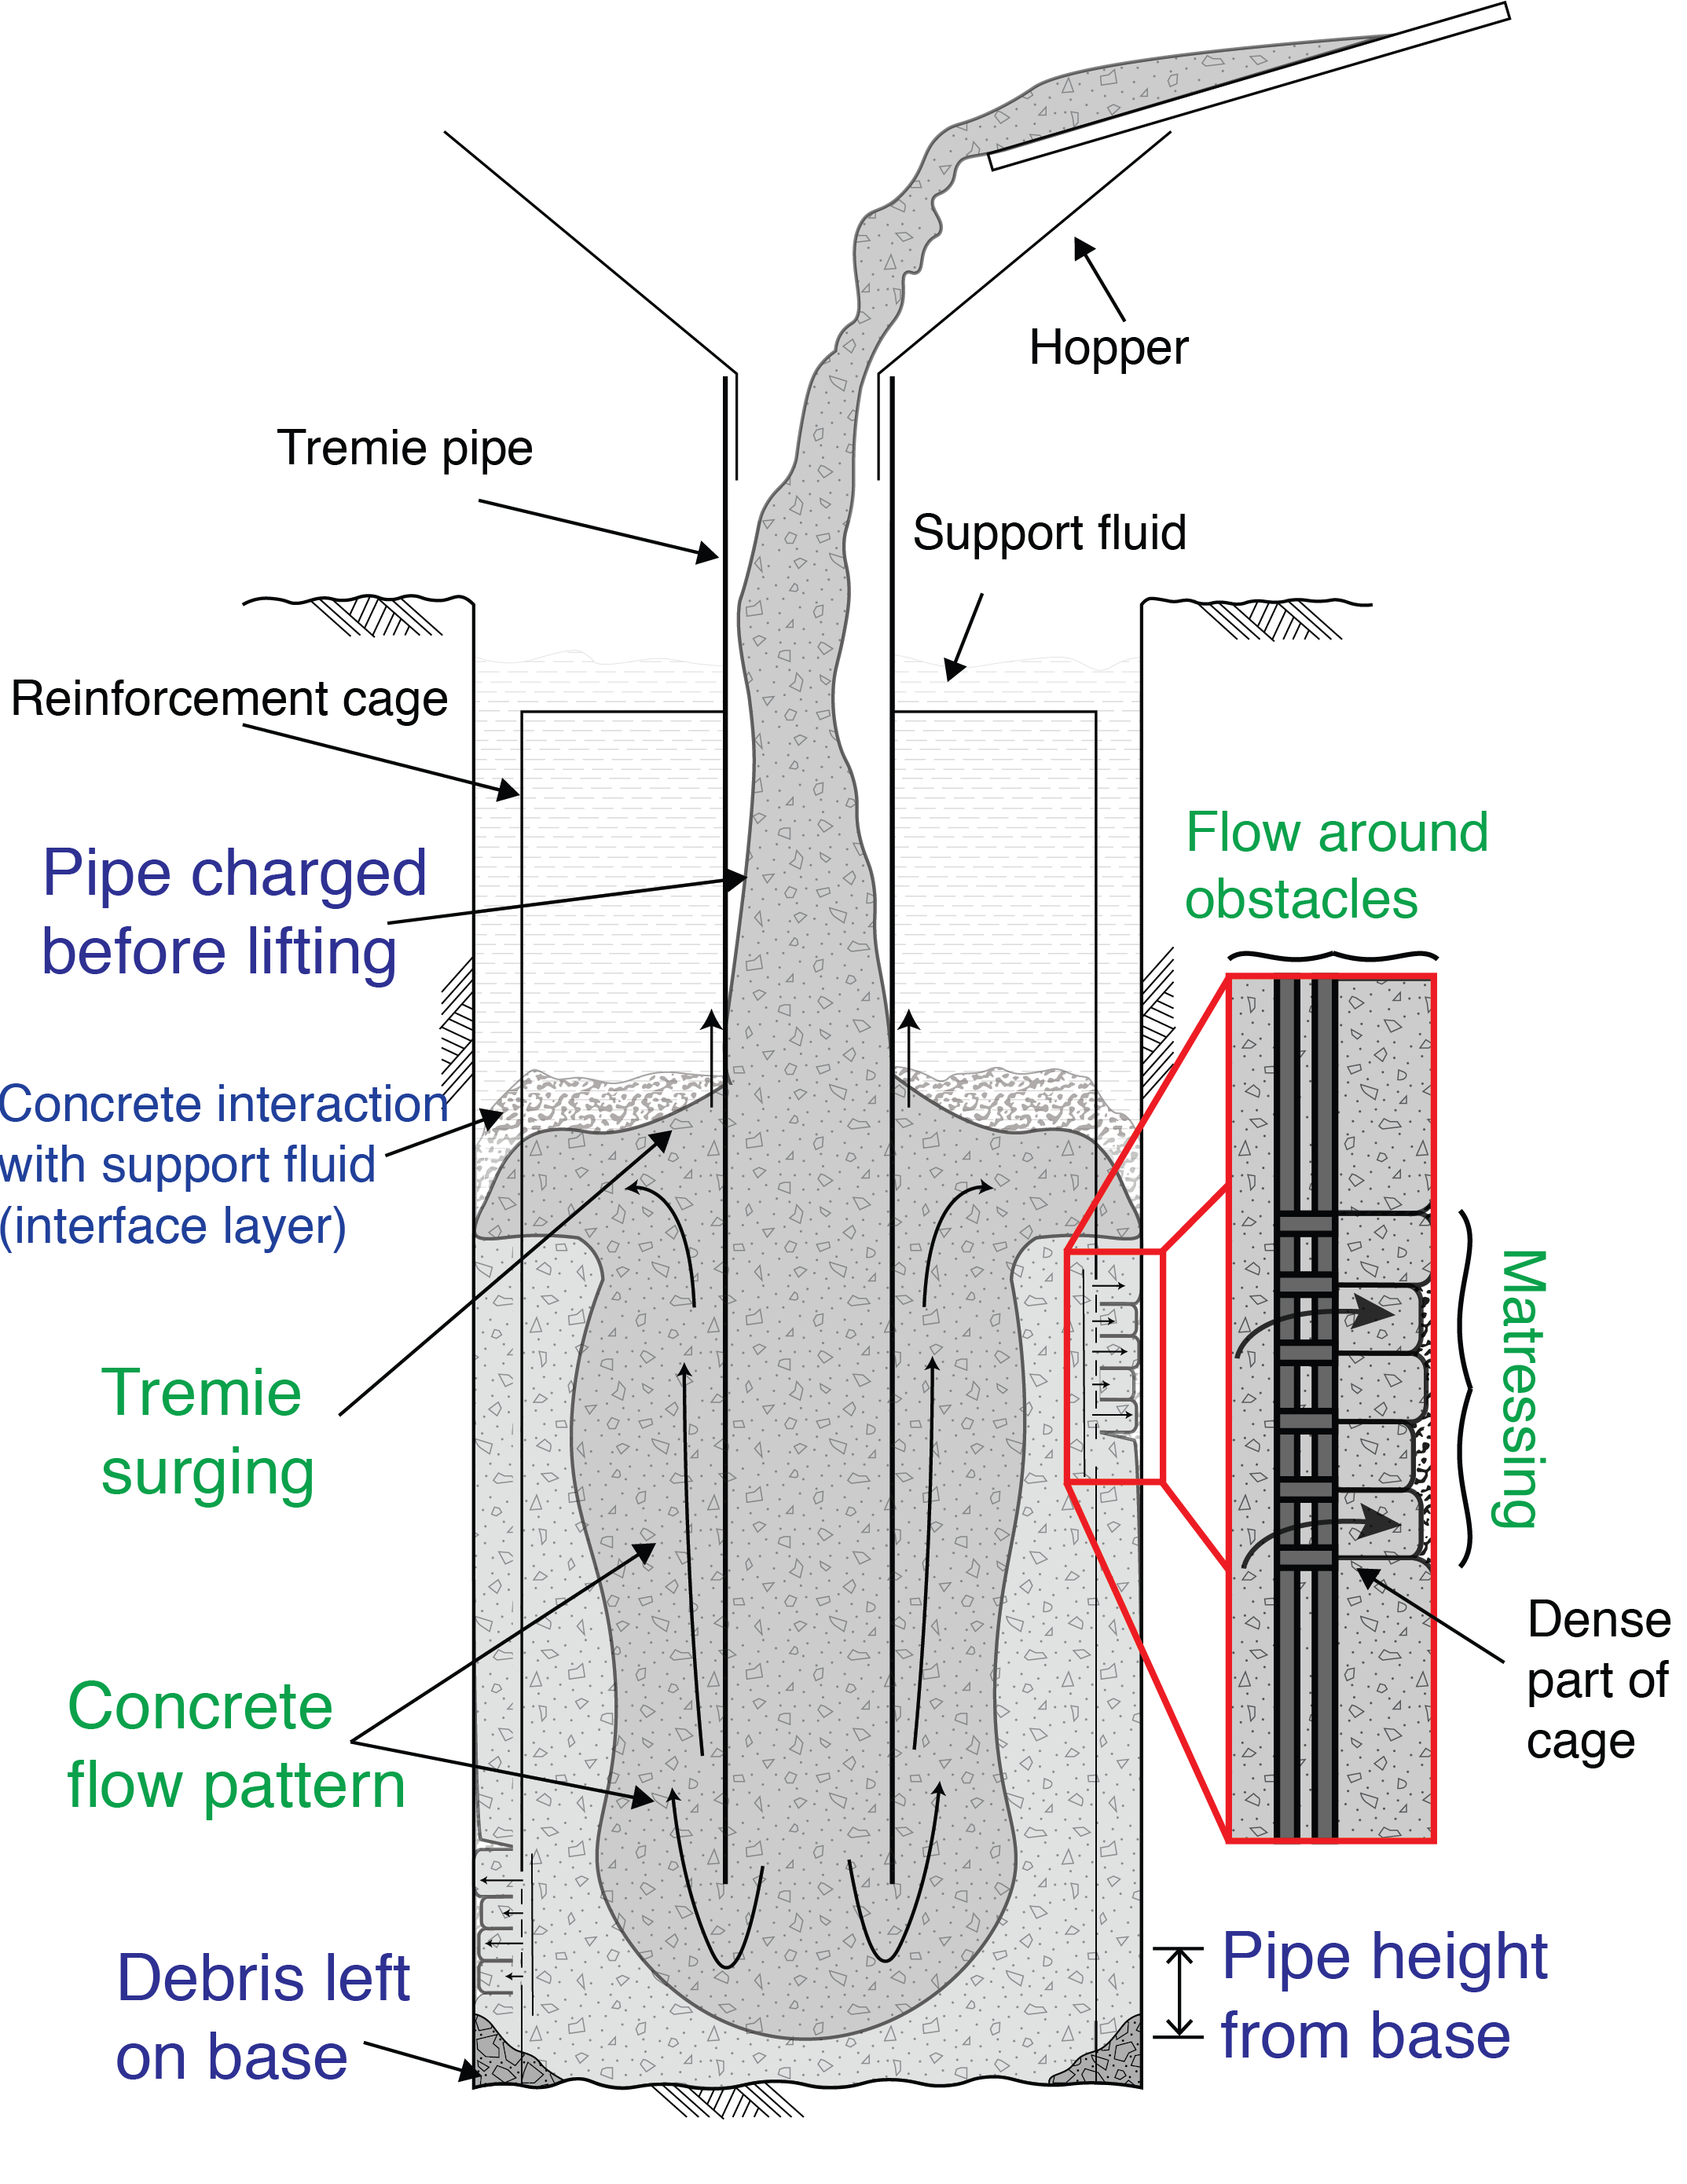
\includegraphics[width=0.65\textwidth]{tremie_colour.png}
\caption{\label{fig:tremie_colour} Schematic diagram of a bored pile cast using tremie method, with areas of investigation highlighted and colour coded.}
\end{figure}


\subsection{Initiation of Concrete Flow}

Areas of investigation related to the initiation of concrete flow are centred around the physical apparatus used in the process and the conditions of the shaft prior to beginning concreting as seen in {\bfseries figure \ref{fig:flow_init}}.\\

\noindent
The importance of base cleaning, demonstrated in {\bfseries figure \ref{fig:flow_init}a}, is reiterated throughout \citeauthor{BS1536}, \citetex{EFFC}, and \citetex{Sperwall}. The need for pile baring capacity to be accurately calculated by relying on the assumption of a smooth base being a primary concern. However, although a smooth base is critical for pile design purposes, \citetex{EFFC} hypothesise that debris from the base can be stirred up and included in the pile. Developing a simulation to assess the degree of inclusions caused by an unclean base could provide advice on whether base cleaning is needed in conditions where end baring capacity is not a critical factor of the pile design.\\

\noindent
{\bfseries
Figure \ref{fig:flow_init}b} and {\bfseries figure \ref{fig:flow_init}c}  demonstrate the initial charging and raising of the tremie to initiate concrete flow. \citetex{Sperwall} recommend raising the pipe to $200mm$ prior to initiation of flow to allow for the prevention of blockages from the initial pour. Both \citetex{Sperwall} and \citetex{EFFC} also recommend the use of a plug to allow the tremie to be filled with concrete prior to initiation. This also allows for the prevention of contamination with support fluid during filling of the pipe. However, little evidence is provided to determine the effectiveness of using such a method. This study aims to simulate varying plugging methods and make a recommendation on the effectiveness of each.\\

\noindent
Finally, {\bfseries figure \ref{fig:flow_init}d}  demonstrates the first 'cut' of the tremie pipe. During concreting, the tremie pipe is periodically raised and a segment unscrewed. This maintains a required embedment of around $3m-8m$ (\citeauthor{BS1536}) throughout the pouring process. In contrast, \citetex{EFFC} recommend for the first cut, an embedment of $5m$ is maintained. Analysing the behaviour of concrete with these contrasting embedment depths can help alleviate some of the contrasting opinions currently surrounding the depth of embedment. Additionally, \citetex{EFFC} and \citetex{Sperwall} also make reference to maintaining a charged pipe such that the hydrostatic pressure inside the pipe is greater than that outside, preventing inflow of the support fluid. Observations of pressure changes within the tremie pipe will be made during the simulation to assess the likelihood of infiltration of support fluid into the tremie pipe.

\begin{figure}[H]
\centering
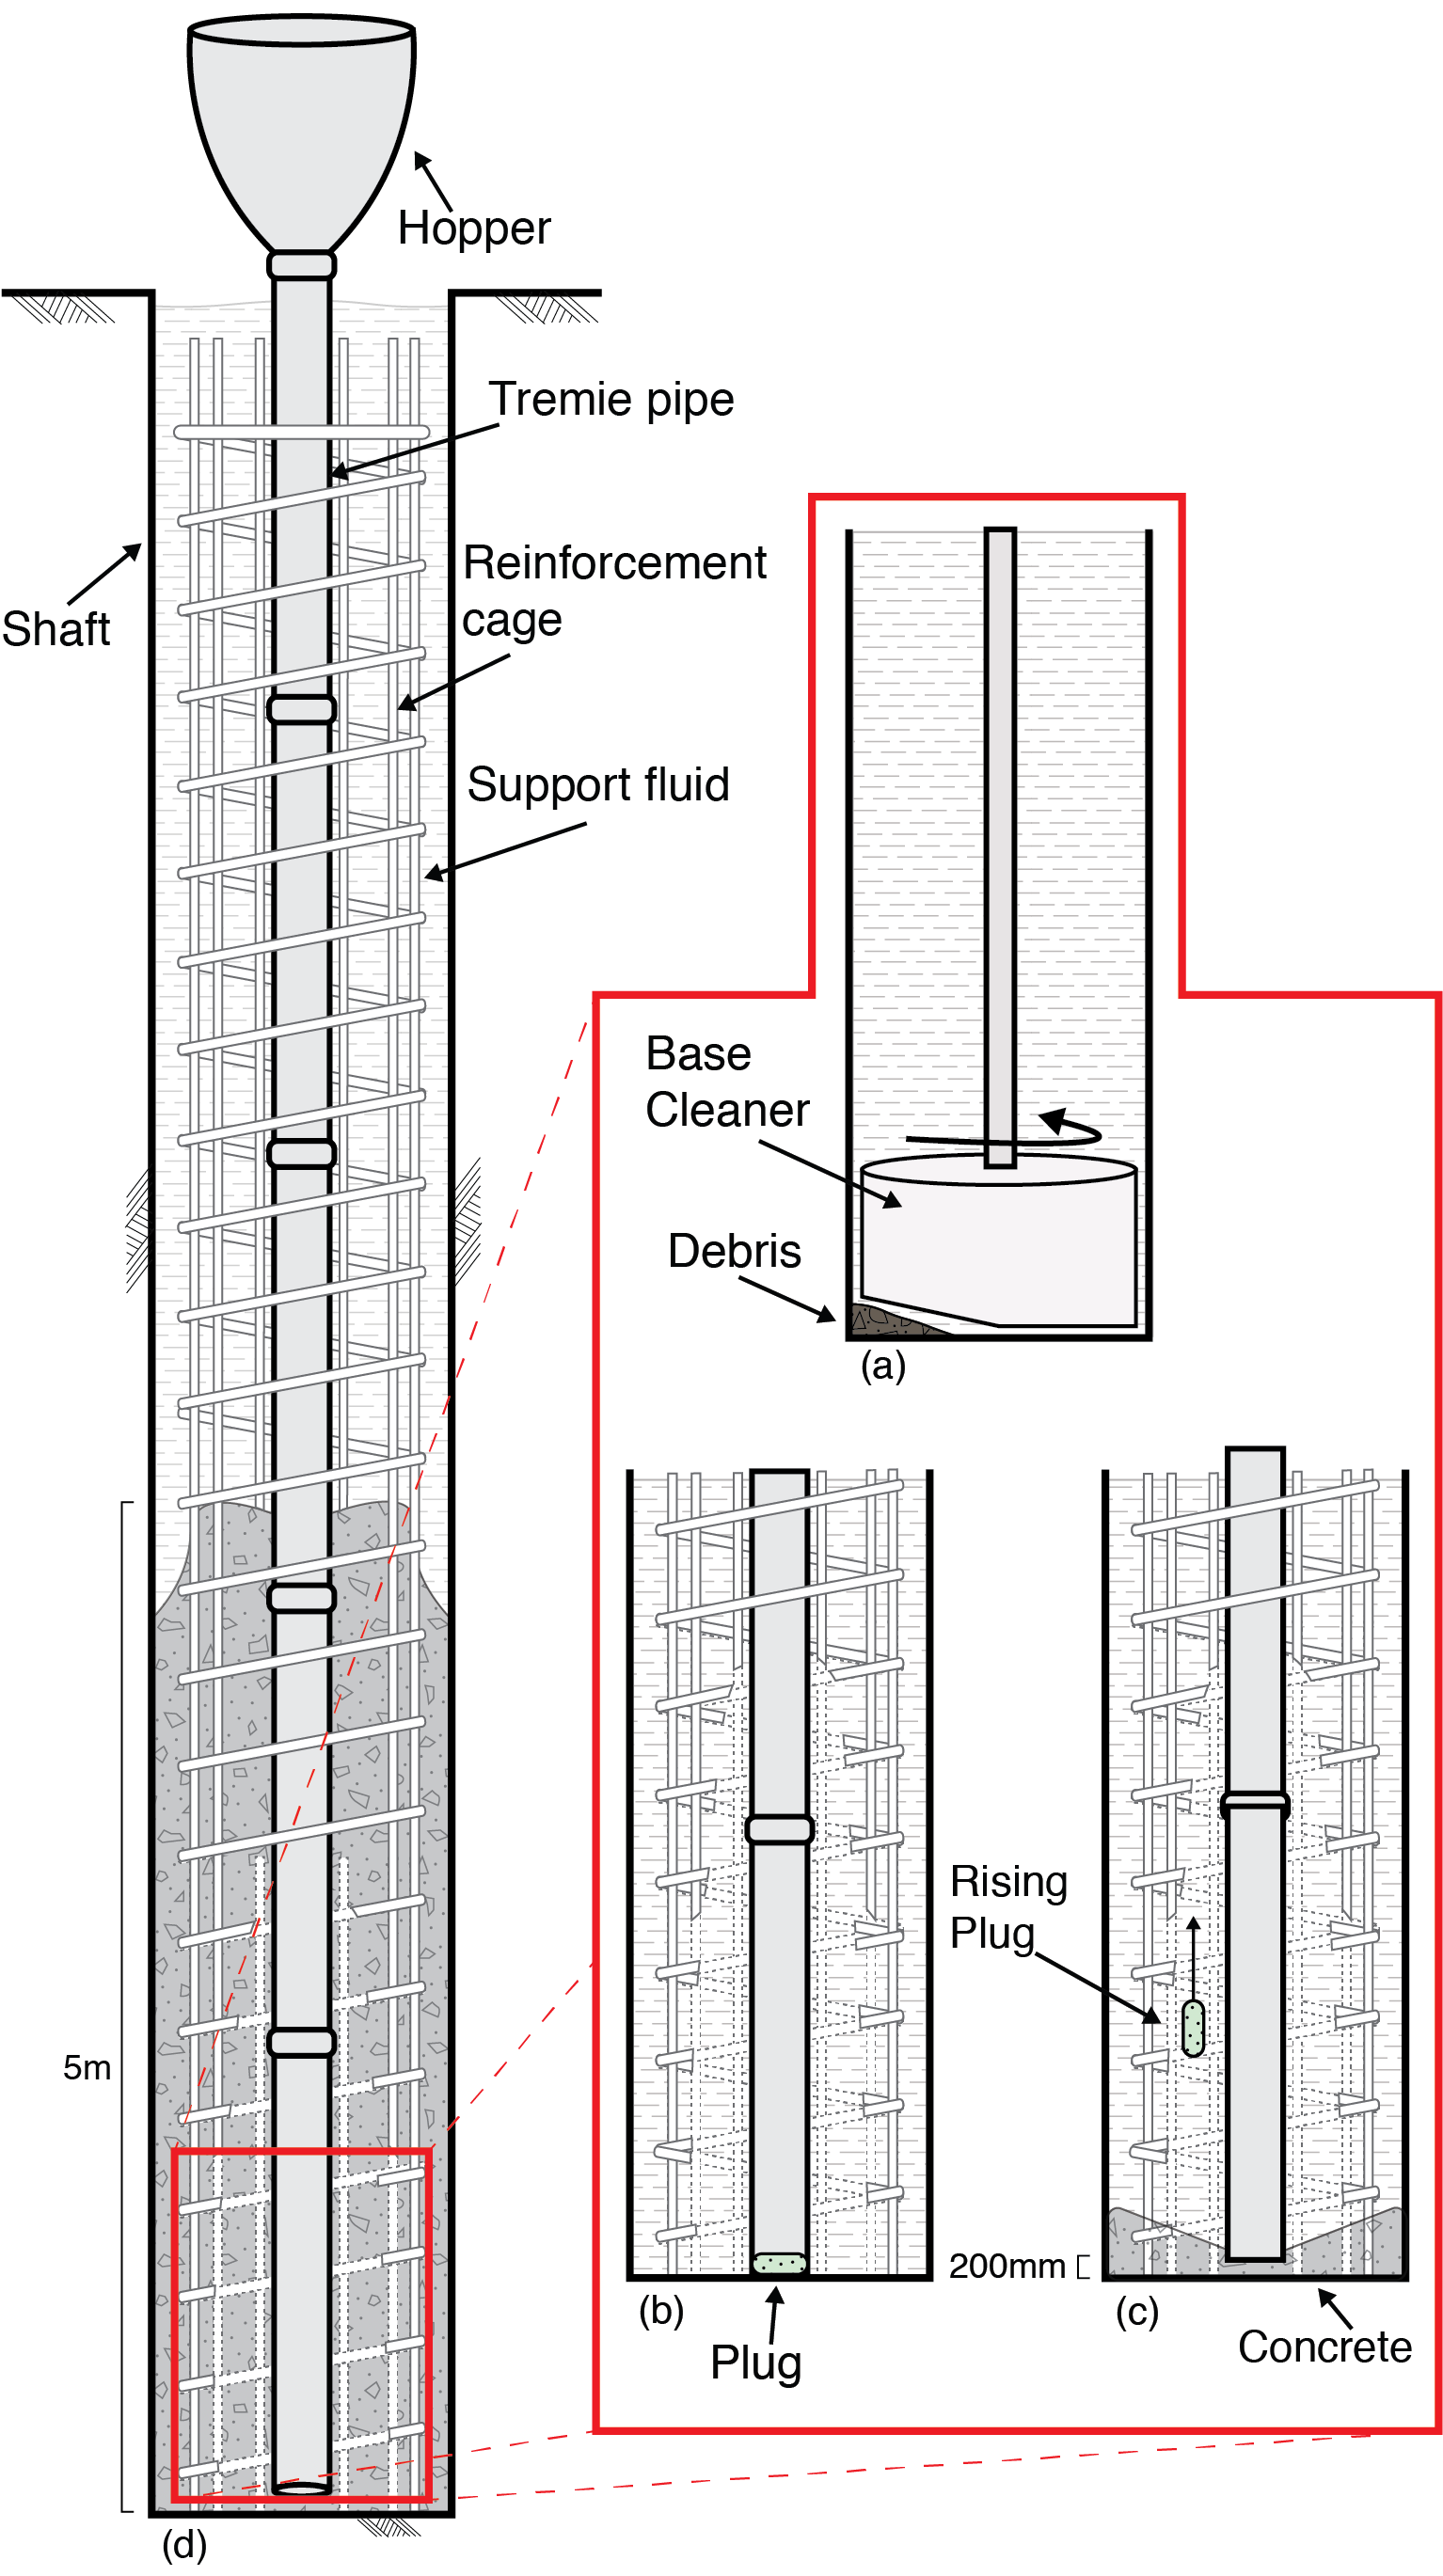
\includegraphics[width=0.8\textwidth]{initial_flow_issues.png}
\caption{\label{fig:flow_init} a) Schematic of base cleaner tool used to create a smooth base in shaft. b)\& c) Schematic showing use of plug or 'pig' to prevent concrete within pipe from free-falling into support fluid. d) Schematic showing required embedment before tremie can be raised.}
\end{figure}

%********************************** During Flow  ****************************
\subsection{During Concrete Flow}

During initiation of flow problems are likely to arise as a result of improper concreting techniques, the same cannot be said for issues that arise during concrete flow; for these issues are more closely related to the material properties of the concrete.\\

\noindent
\citetex{Sperwall} and \citetex{EFFC} emphasise that concrete should flow freely from the tremie pipe without the need for surging (lowering and raising the pipe to facilitate flow). Although flowing freely is a requirement, little is understood about the manner in which the concrete flows. \citetex{EFFC} describes the the various theorised methods of the flowing of concrete out of the tremie pipe and into the surrounding shaft as varying 'flow patterns'. There are two main theorised flow patterns, 'plug flow' and 'volcano flow' as demonstrated in {\bfseries figure XX}. Each flow pattern has an impact on the required open-life of the concrete; plug flow requiring the lengthier open-life. Achieving a longer open life requires the potential introduction of superplasticizers and retarders, both of which come at an increased cost and often a lack of understanding. Therefore, determining the dominant flow pattern through simulations could help provide advice on concrete open-life.\\

\noindent
A congested reinforcement cage can give rise to poor coverage of concrete, in contrast there are cases where a seemingly uncongested cage has induced a defect termed 'matressing'. This occurs as a result of concrete poorly flowing around the rebars of a reinforcement cage, as demonstrated in {\bfseries figure \ref{fig:matress}a \& b}. \citet{EFFC} infer the implications of such imperfections could cause pathways bleed water, reductions in bearing capacity, and durability concerns. Developing a series of simulations to predict the likelihood of matressing occurring will generate useful insights into both how reinforcement cages are designed and how important the material properties of the concrete are in reducing matressing.It is also suggested that a reduction in hydrostatic pressure towards the top of the pile may exacerbate this problem, which will be investigated.\\

\noindent
\citeauthor{BS1536} recommends the use of a support fluid such as bentonite for preventing collapse of the shaft during drilling and casting of foundations. Although a fundamental part of the casting in situ process, it is not without complications, {\bfseries figure \ref{fig:matress}c}. It is observed during casting that atop the rising concrete with the pile will be an interface layer; a mixture of support fluid and concrete. This low strength material could possibly be enveloped by concrete to form an inclusion, particularly in the cover zone. Investigating how this material flows through a pile may shed light on what is currently a poorly understood by-product of using bentonite support fluid. 


\begin{figure}[H]
\centering
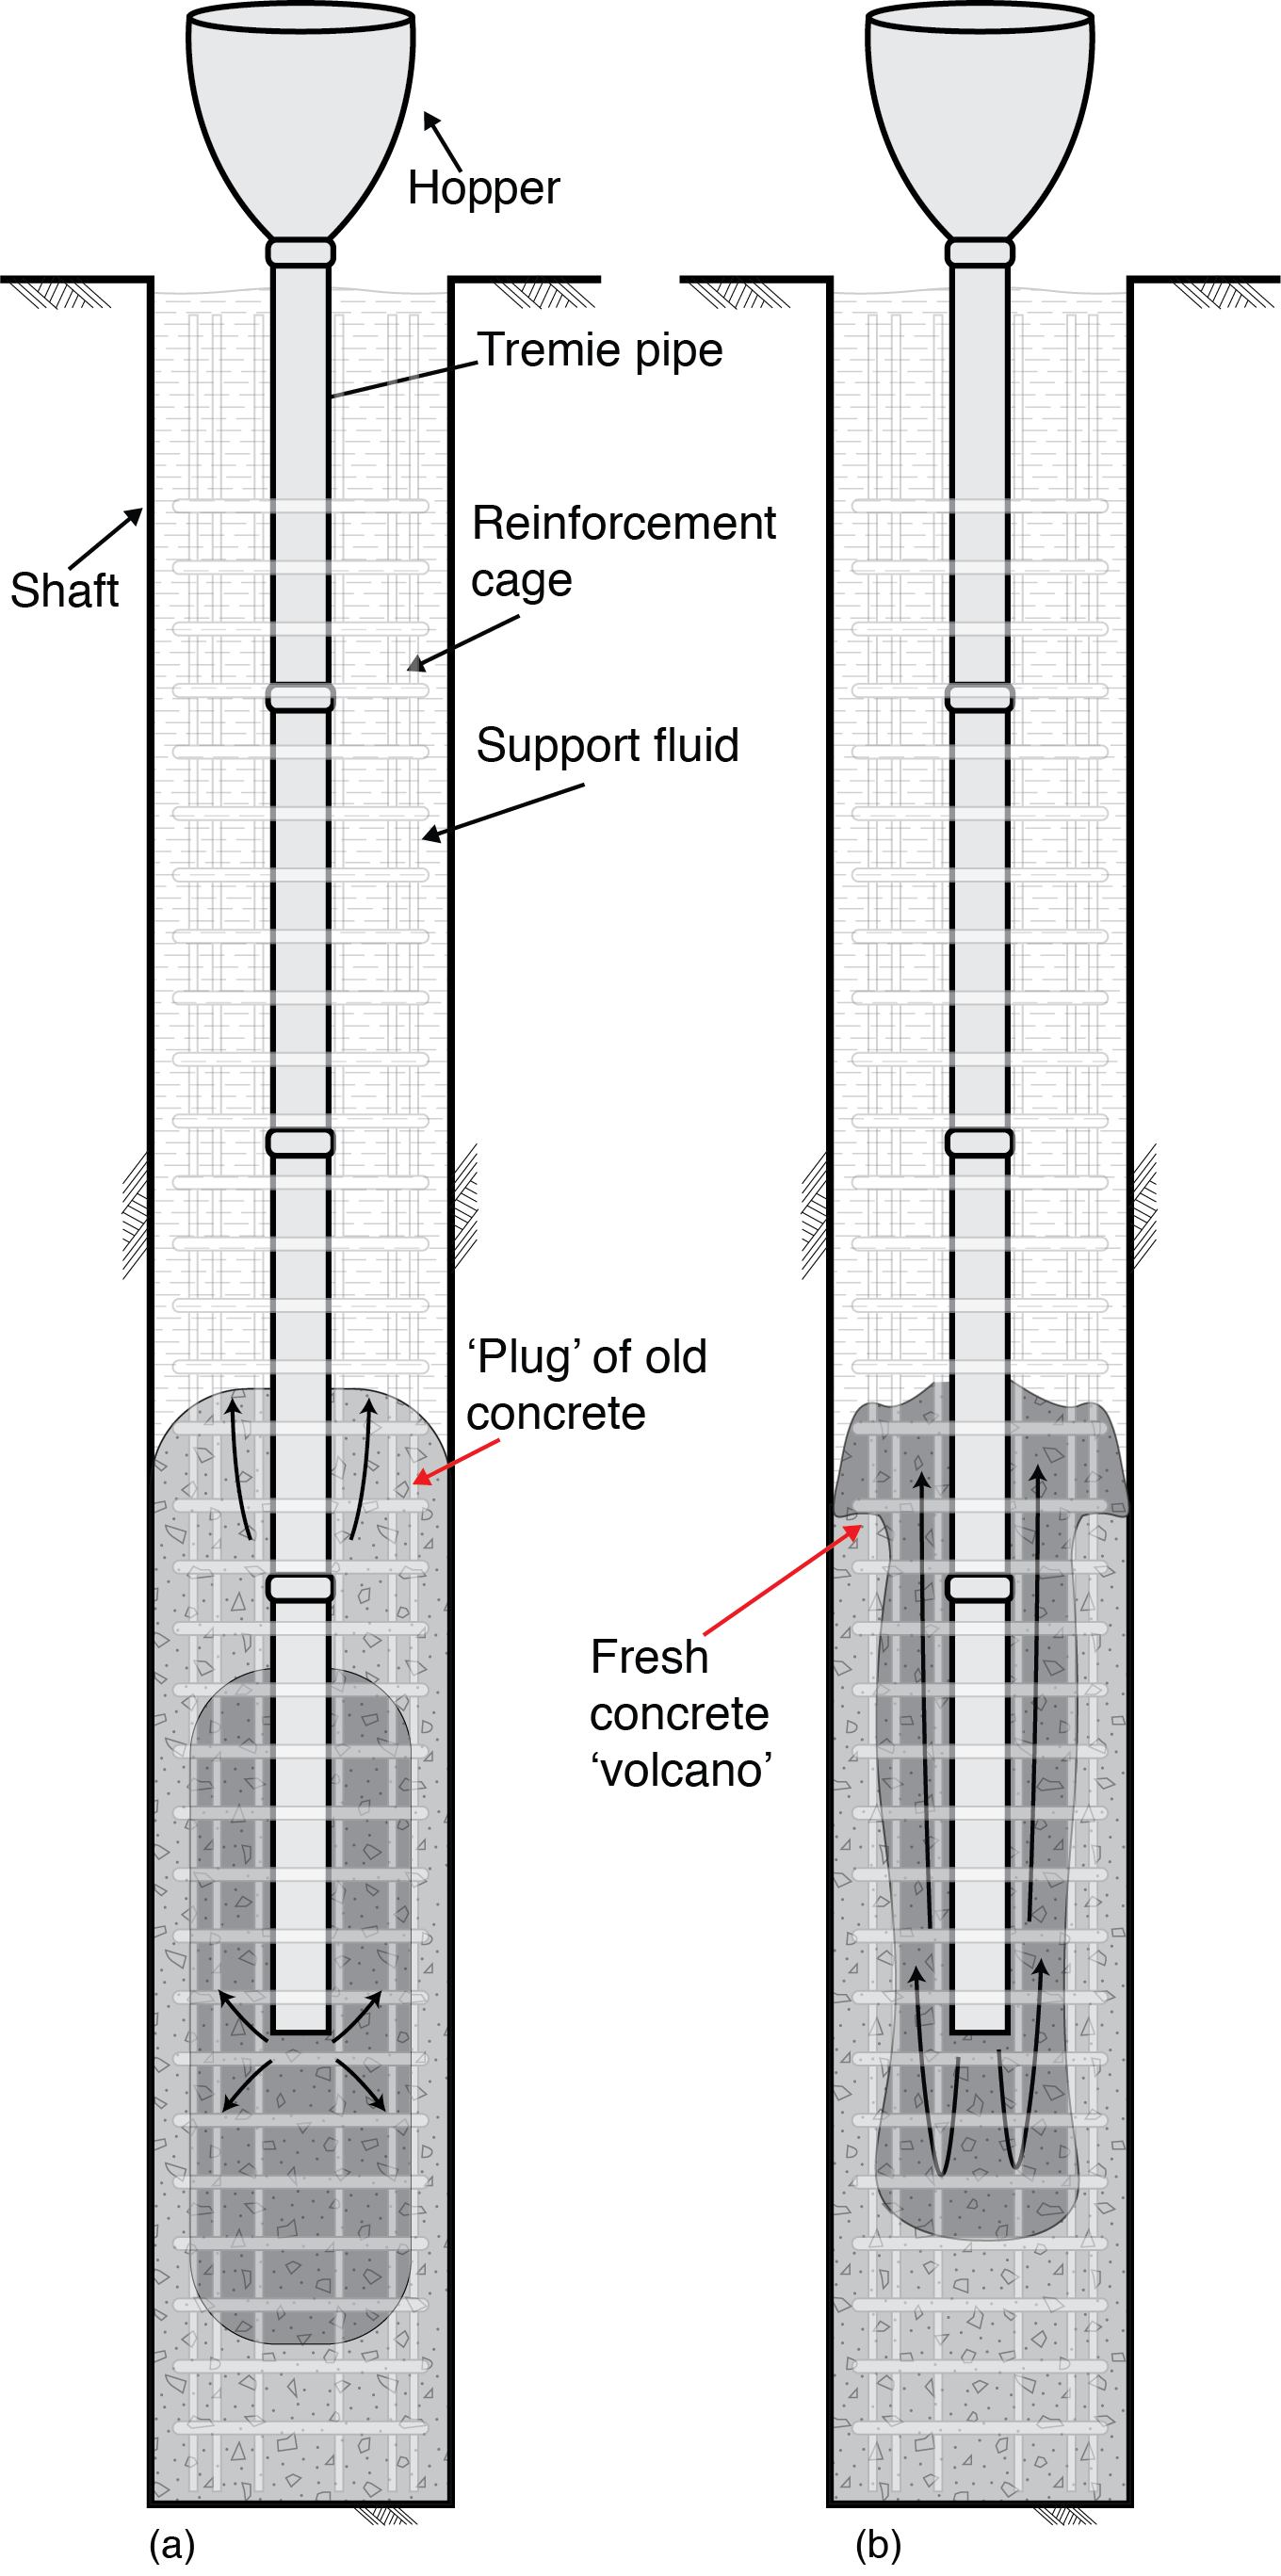
\includegraphics[width=0.7\textwidth]{flow_pattern_newstyle.png}
\caption{\label{fig:flowpattern}Schematic pile diagram showing a) theorised plug flow, where old concrete rises above fresh, and b) fresh concrete erupting at surface, referred to as volcano flow.}
\end{figure}

\begin{figure}[H]
\centering
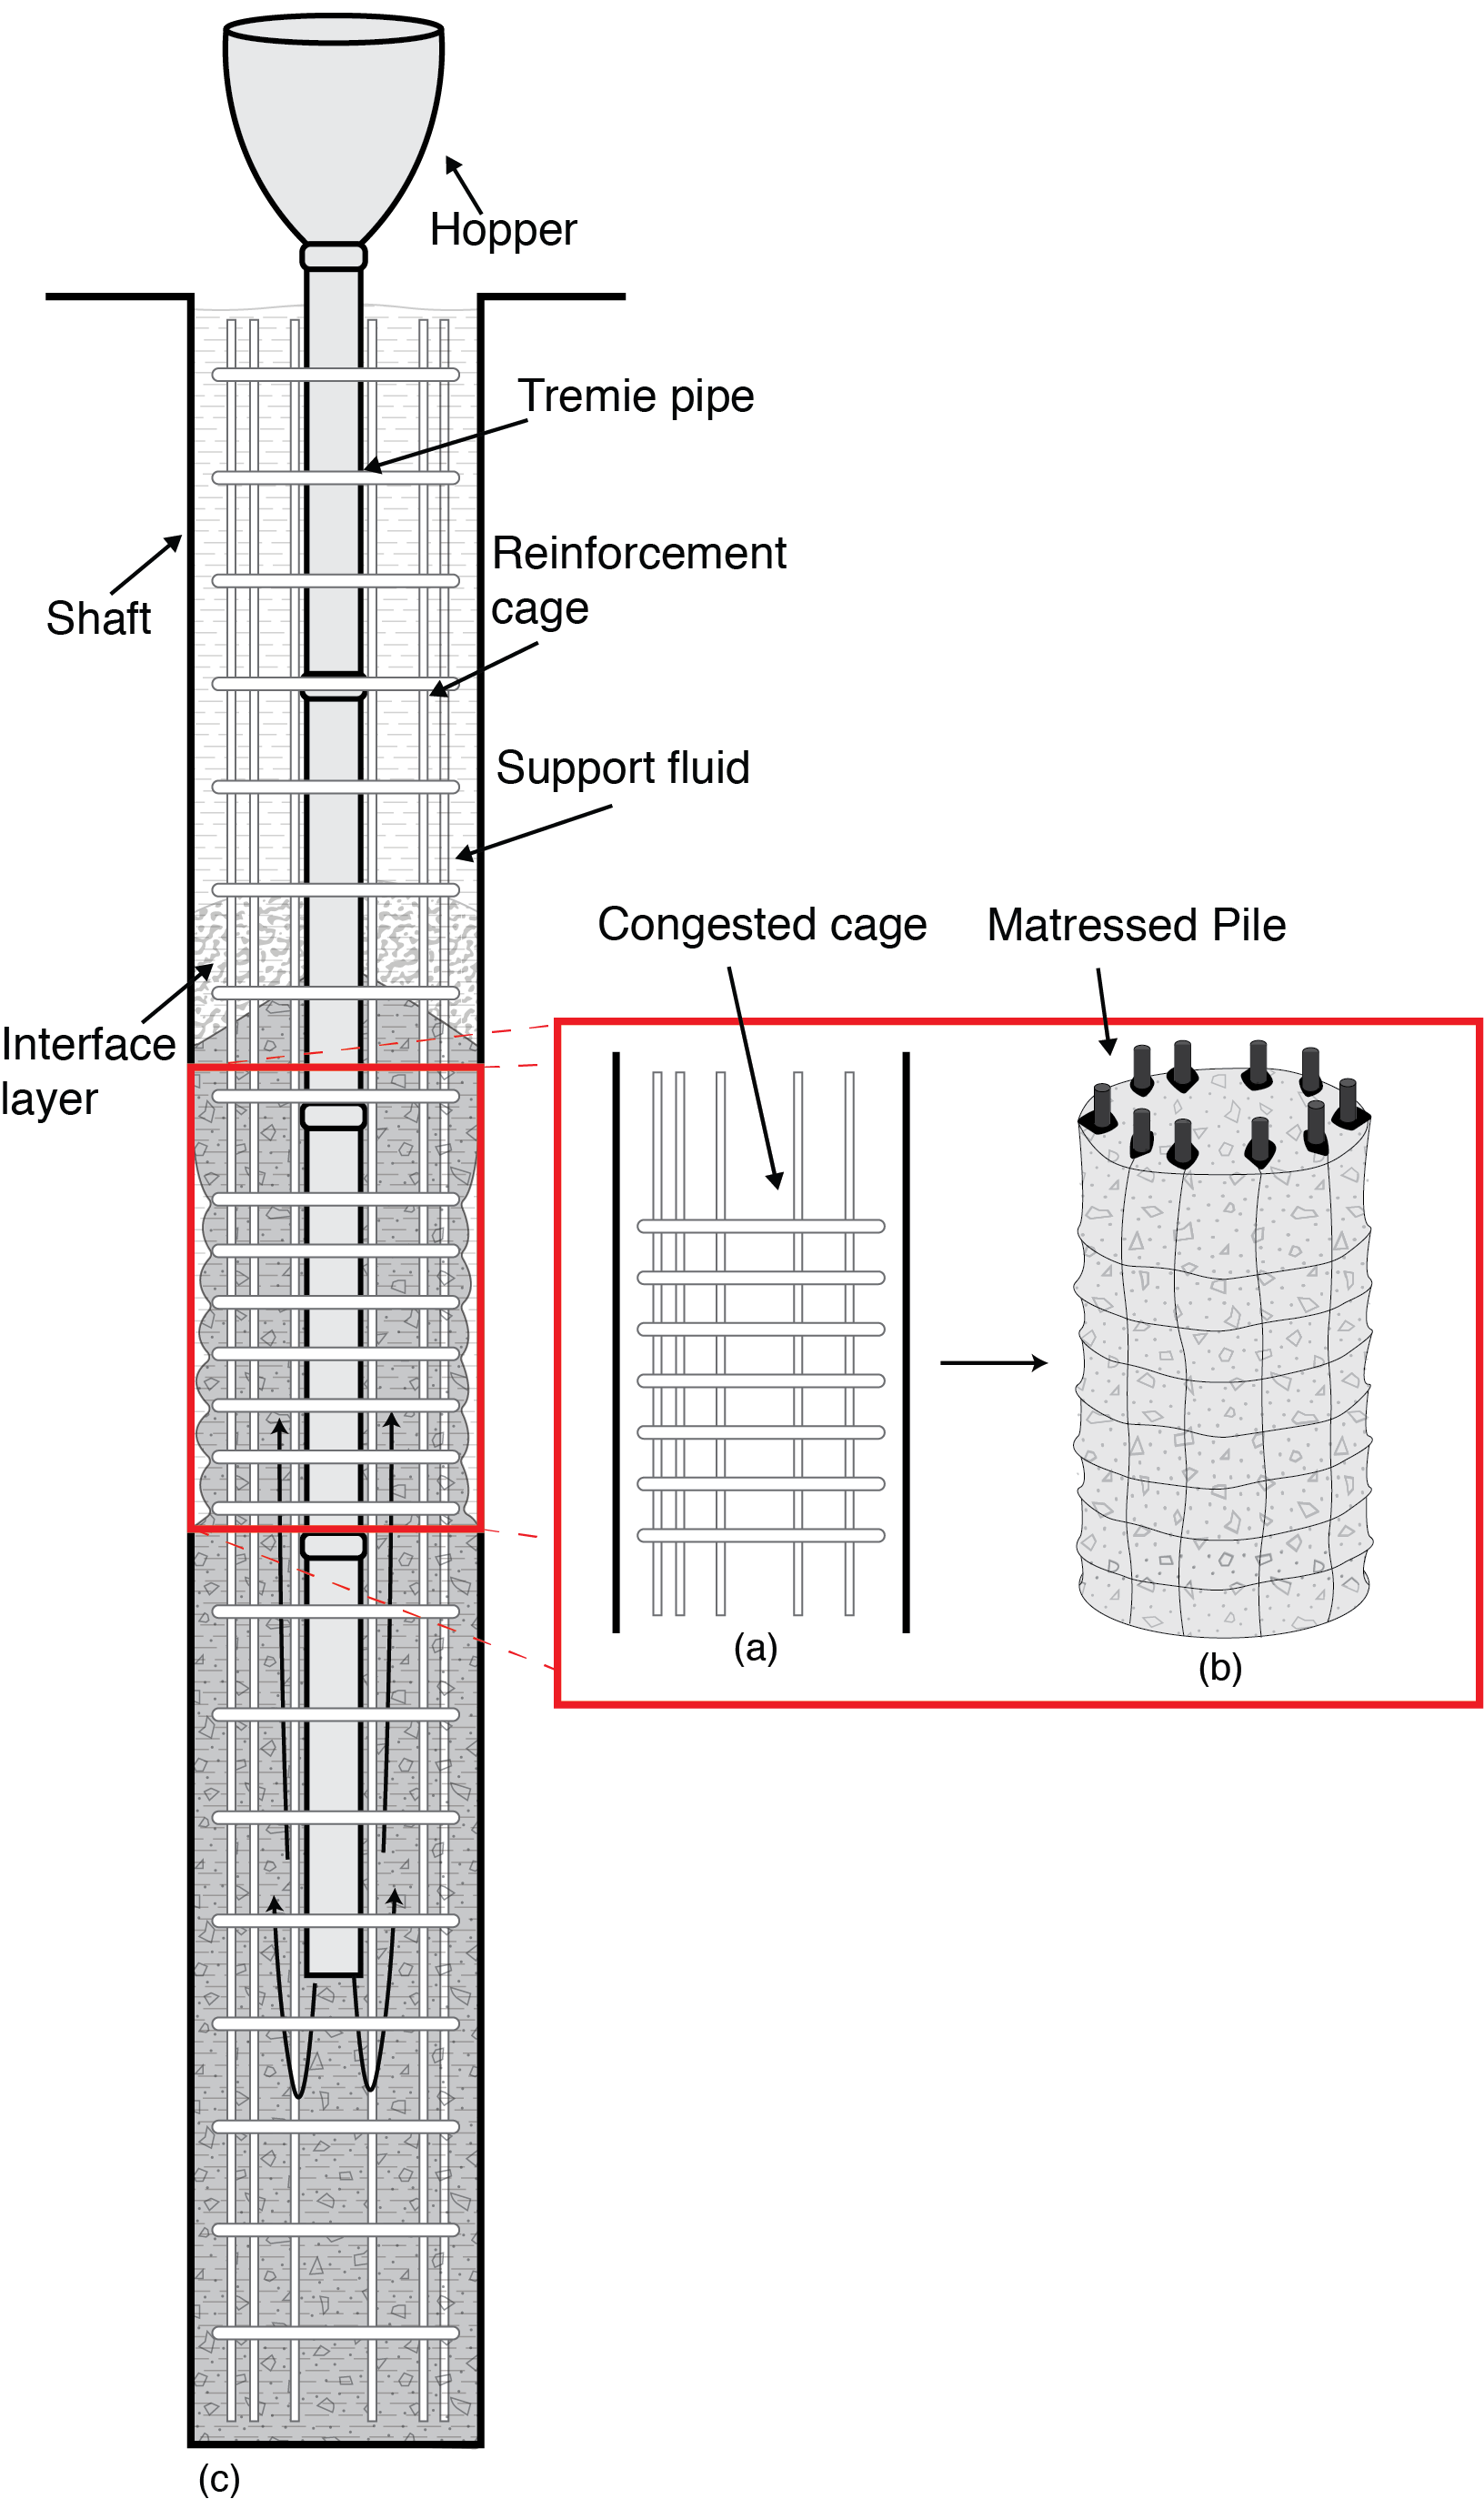
\includegraphics[width=0.8\textwidth]{matress.png}
\caption{\label{fig:matress}Diagram showing how a congested cage (a) could lead to a matressing effect on a a pile (b). c) Demonstrates that matressing likely to occur towards top of pile due to reduction in hydrostatic pressure.}
\end{figure}

\subsection{Bleed and Segregation}

Bleed and segregation issues within a cast in situ deep foundation can be extremely detrimental to the foundation. Mitigating the development of bleed within a pile should be a primary concern for the contractor, to prevent segregation occurring. Nonetheless, establishing when bleed has occurred or will occur is contentious. \citetex{EFFC} stipulates measures should be taken to avoid bleed and segregation, suggesting the material properties of the concrete have a direct baring on the likelihood of segregation. Simulations of varying properties may help provide guidance on acceptance criteria for concrete such that the effects of bled and segregation could be minimised.









